\documentclass[12pt]{article}

\usepackage[utf8]{inputenc}
\usepackage[swedish,english]{babel}
\usepackage{tikz}
\usepackage{amsmath}
\usepackage{subfiles}
\usepackage{calc}
\usepackage{graphicx}
\DeclareGraphicsExtensions{.eps,.pdf,.png,.jpg}
\graphicspath{{images/}}
\usetikzlibrary{calc, shapes, arrows, chains, positioning, matrix, scopes, shadows}

% Define some styles to use with tikz
\tikzstyle{cloud}     = [ellipse, draw, fill=blue!30, node distance=40pt,minimum height=20pt]
\tikzstyle{state}     = [ellipse, draw, fill=violet!30, node distance=40pt,minimum height=20pt]
\tikzstyle{subbyte}   = [rectangle, draw, text width=100pt, text centered, rounded corners=10pt, minimum height=20pt, fill=red!30]
\tikzstyle{shiftrow}  = [rectangle, draw, text width=100pt, text centered, rounded corners=10pt, minimum height=20pt, fill=orange!30]
\tikzstyle{mixcolumn} = [rectangle, draw, text width=100pt, text centered, rounded corners=10pt, minimum height=20pt, fill=yellow!30]
\tikzstyle{roundkey}  = [rectangle, draw, text width=100pt, text centered, rounded corners=10pt, minimum height=20pt, fill=green!30]
\tikzstyle{line} = [draw, -latex']

\title{AES Encryption in FPGA hardware}
\foreignlanguage{swedish}{
\author{
        Patrik Dahlström \\
        Electronic Design\\
            \and
        Daniel Josefsson\\
        Electronic Design\\
            \and
        Staffan Sjöqvist\\
        Electronic Design
}
}
\date{\today}

\begin{document}
\maketitle

\begin{abstract}
Some abstract
\end{abstract}

\pagebreak

\section{Introduction}
AES encryption is a widely recognized standard encryption that is well used in many modern applications of today. It can be found not only in modern wireless network, but also in encryption devices designed for secure storage as well as in secure wired networks.

It is this group's intention to learn how this encryption works and also how to implement it in FPGA hardware.

\subfile{definitions.tex}

\section{Theory} \label{sec:theory}
The AES encryption process can be divided in two different sections:
\begin{itemize}
\item Encryption process
\item Key schedule
\end{itemize}
In encryption process, an unencrypted data packet is encrypted using a cipher key and in key schedule the different round keys needed for the encryption process are generated.

\subfile{encryption_process.tex}

\subfile{key_schedule.tex}

\section{Timeline}\label{timeline}
%The timeline below is graded in number of weeks from project start

\begin{figure}[h]
\centering
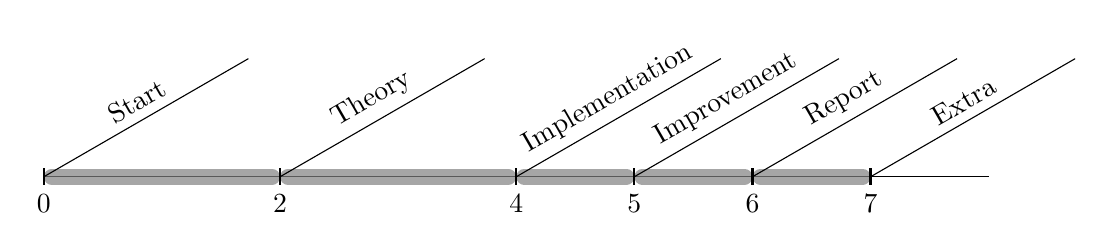
\begin{tikzpicture}
% Draw horizontal lines
\foreach \x/\y in {0/3,3/6,6/7.5,7.5/9,9/10.5,10.5/12}
    \draw (\x,0) -- (\y,0);

% Draw horizontal lines (thicker, transparent)
\foreach \x/\y in {0/3,3/6,6/7.5,7.5/9,9/10.5}
    \draw[line width=2mm,gray,line cap=round,opacity=0.7] (\x+0.1,0) -- (\y-0.1,0);

% Draw vertical lines
\foreach \x in {0,3,6,7.5,9,10.5}
   \draw[thick] (\x cm,3pt) -- (\x cm,-3pt);

% Put in weeks
\foreach \x/\xweek in {0/0,3/2,6/4,7.5/5,9/6,10.5/7}
   \draw (\x,0) node[below=3pt]{\xweek};
   
% Add slanted labels for each week
\foreach \x/\text in {0/{Start},
                      3/{Theory},
                      6/{Implementation},
                      7.5/{Improvement},
                      9/{Report},
                      10.5/{Extra}}
    \draw (\x,0) -- +(30:3) node[midway,sloped,above]{\text};

\end{tikzpicture}
\caption{Timeline in project weeks}
\end{figure}

\end{document}
